\documentclass[12pt, letterpaper]{article}
\pdfminorversion=4
\usepackage[utf8]{inputenc}
\usepackage{textcomp}
\usepackage{listings}
\usepackage{babel}
\usepackage[square,numbers]{natbib}
%\usepackage{amsmath}
\usepackage{amssymb,amsmath,amsthm,amsfonts}
\usepackage{adjustbox}
\usepackage{pslatex}
%\usepackage{bm}% better \boldsymbol
\usepackage{array}% improves tabular environment.
\usepackage{dcolumn}% also improves tabular environment, with decimal centring.
%\usepackage{lastpage}
\usepackage{listings}
\usepackage{tikz}
\usetikzlibrary{decorations.pathmorphing}
%\usepackage{pgfplots}
%\usepackage{cleveref}
\usepackage{pgf,pgfarrows,pgfnodes}

\usepackage[final]{pdfpages}
\usepackage{hyperref}
\usepackage{doi}
\usepackage{mathrsfs}

%\usepackage[altbullet,expert]{lucidabr}
%\usepackage[charter]{mathdesign}
\usepackage{cleveref}
\usepackage{ifthen}
%\usepackage{nomencl}
\usepackage{parskip}
\usepackage{psfrag}
\usepackage{booktabs}
\usepackage{pifont}
%\usepackage{subfig,caption}
\usepackage{microtype}% for pdflatex; medisin mot overfull \vbox
\usepackage{xspace}% for pdflatex; medisin mot overfull \vbox
\usepackage[font=footnotesize]{subcaption}
\usepackage{siunitx}
\usepackage{todonotes}
\presetkeys%
    {todonotes}%
    {inline,backgroundcolor=orange}{}

%% Formattering av figur- og tabelltekster
%
%
% Egendefinerte
%
%\newcommand*{\od}[3][]{\frac{\mathrm{d}^{#1}#2}{\mathrm{d}{#3}^{#1}}}% ordinary derivative
\newcommand*{\od}[3][]{\frac{\dif^{#1}#2}{\dif{#3}^{#1}}}% ordinary derivative
\newcommand*{\pd}[3][]{\frac{\partial^{#1}#2}{\partial{#3}^{#1}}}% partial derivative
\newcommand*{\pdt}[3][]{{\partial^{#1}#2}/{\partial{#3}^{#1}}}% partial
                                % derivative for inline use.
\newcommand{\pone}[3]{\frac{\partial #1}{\partial #2}_{#3}}% partial
                                % derivative with information of
                                % constant variables
\newcommand{\ponel}[3]{\frac{\partial #1}{\partial #2}\bigg|_{#3}} % partial derivative with informatio of constant variable. A line is added.
\newcommand{\ptwo}[3]{\frac{\partial^{2} #1}{\partial #2 \partial
    #3}} % partial differential in two different variables
\newcommand{\pdn}[3]{\frac{\partial^{#1}#2}{\partial{#3}^{#1}}}% partial derivative

% Total derivative:
\newcommand*{\ttd}[2]{\frac{\mathrm{D} #1}{\mathrm{D} #2}}
\newcommand*{\td}[2]{\frac{\mathrm{d} #1}{\mathrm{d} #2}}
\newcommand*{\ddt}{\frac{\partial}{\partial t}}
\newcommand*{\ddx}{\frac{\partial}{\partial x}}
% Vectors etc:
% For Computer Modern:

\DeclareMathAlphabet{\mathsfsl}{OT1}{cmss}{m}{sl}
%\renewcommand*{\vec}[1]{\boldsymbol{#1}}%
\newcommand*{\vc}[1]{\vec{\mathbf{#1}}}%
\newcommand*{\tensor}[1]{\mathsfsl{#1}}% 2. order tensor
\newcommand*{\matr}[1]{\tensor{#1}}% matrix
\renewcommand*{\div}{\boldsymbol{\nabla\cdot}}% divergence
\newcommand*{\grad}{\boldsymbol{\nabla}}% gradient
% fancy differential from Claudio Beccari, TUGboat:
% adjusts spacing automatically
\makeatletter
\newcommand*{\dif}{\@ifnextchar^{\DIfF}{\DIfF^{}}}
\def\DIfF^#1{\mathop{\mathrm{\mathstrut d}}\nolimits^{#1}\gobblesp@ce}
\def\gobblesp@ce{\futurelet\diffarg\opsp@ce}
\def\opsp@ce{%
  \let\DiffSpace\!%
  \ifx\diffarg(%
    \let\DiffSpace\relax
  \else
    \ifx\diffarg[%
      \let\DiffSpace\relax
    \else
      \ifx\diffarg\{%
        \let\DiffSpace\relax
      \fi\fi\fi\DiffSpace}
\makeatother
%
\newcommand*{\me}{\mathrm{e}}% e is not a variable (2.718281828...)
%\newcommand*{\mi}{\mathrm{i}}%  nor i (\sqrt{-1})
\newcommand*{\mpi}{\uppi}% nor pi (3.141592...) (works for for Lucida)
%
% lav tekst-indeks/subscript/pedex
\newcommand*{\ped}[1]{\ensuremath{_{\text{#1}}}}
% hy tekst-indeks/superscript/apex
\newcommand*{\ap}[1]{\ensuremath{^{\text{#1}}}}
\newcommand*{\apr}[1]{\ensuremath{^{\mathrm{#1}}}}
\newcommand*{\pedr}[1]{\ensuremath{_{\mathrm{#1}}}}
%
\newcommand*{\volfrac}{\alpha}% volume fraction
\newcommand*{\surften}{\sigma}% coeff. of surface tension
\newcommand*{\curv}{\kappa}% curvature
\newcommand*{\ls}{\phi}% level-set function
\newcommand*{\ep}{\Phi}% electric potential
\newcommand*{\perm}{\varepsilon}% electric permittivity
\newcommand*{\visc}{\mu}% molecular (dymamic) viscosity
\newcommand*{\kvisc}{\nu}% kinematic viscosity
\newcommand*{\cfl}{C}% CFL number

% Grid
\newcommand{\jj}{j}
\newcommand{\jph}{{j+1/2}}
\newcommand{\jmh}{{j-1/2}}
\newcommand{\jp}{{j+1}}
\newcommand{\jm}{{j-1}}
\newcommand{\nn}{n}
\newcommand{\nph}{{n+1/2}}
\newcommand{\nmh}{{n-1/2}}
\newcommand{\np}{{n+1}}
%
\newcommand{\lf}{\text{LF}}
\newcommand{\lw}{\text{Ri}}
%
\newcommand*{\cons}{\vec U}
\newcommand*{\flux}{\vec F}
\newcommand*{\dens}{\rho}
\newcommand*{\svol}{\ensuremath v}
\newcommand*{\temp}{\ensuremath T}
\newcommand*{\vel}{\ensuremath u}
\newcommand*{\mom}{\dens\vel}
\newcommand*{\toten}{\ensuremath E}
\newcommand*{\inten}{\ensuremath e}
\newcommand*{\press}{\ensuremath p}
\renewcommand*{\ss}{\ensuremath a}
\newcommand*{\jac}{\matr A}
%
\newcommand*{\abs}[1]{\lvert#1\rvert}
\newcommand*{\bigabs}[1]{\bigl\lvert#1\bigr\rvert}
\newcommand*{\biggabs}[1]{\biggl\lvert#1\biggr\rvert}
\newcommand*{\norm}[1]{\lVert#1\rVert}
%
\newcommand*{\e}[1]{\times 10^{#1}}
\newcommand*{\ex}[1]{\times 10^{#1}}%shorthand -- for use e.g. in tables
\newcommand*{\exi}[1]{10^{#1}}%shorthand -- for use e.g. in tables
\newcommand*{\nondim}[1]{\ensuremath{\mathit{#1}}}% italic iflg. ISO. (???)
\newcommand*{\rey}{\nondim{Re}}
\newcommand*{\acro}[1]{\textsc{\MakeLowercase{#1}}}%acronyms etc.

\newcommand{\nto}{\ensuremath{\mbox{N}_{\mbox{\scriptsize 2}}}}
\newcommand{\chfire}{\ensuremath{\mbox{CH}_{\mbox{\scriptsize 4}}}}
%\newcommand*{\checked}{\ding{51}}
\newcommand{\coto}{\ensuremath{\text{CO}_{\text{\scriptsize 2}}}}
\newcommand{\celsius}{\ensuremath{^\circ\text{C}}}
%\newcommand{\clap}{Clapeyron~}
\newcommand{\subl}{\ensuremath{\text{sub}}}
\newcommand{\spec}{\text{spec}}
\newcommand{\sat}{\text{sat}}
\newcommand{\sol}{\text{sol}}
\newcommand{\liq}{\text{liq}}
\newcommand{\vap}{\text{vap}}
\newcommand{\amb}{\text{amb}}
\newcommand{\tr}{\text{tr}}
\newcommand{\crit}{\text{crit}}
\newcommand{\entr}{\ensuremath{\text{s}}}
\newcommand{\fus}{\text{fus}}
\newcommand{\flash}[1]{\ensuremath{#1\text{-flash}}}
\newcommand{\spce}[2]{\ensuremath{#1\, #2\text{ space}}}
\newcommand{\spanwagner}{\text{Span--Wagner}}
\newcommand{\triplepoint}{\text{TP triple point}}
\newcommand{\wrpt}{\text{with respec to~}}
%\sisetup{input-symbols = {( )}}
% \newcommand*{\red}{\ensuremath{\text{R}}\xspace}
% \newcommand*{\crit}{\ensuremath{\text{c}}\xspace}
% \newcommand*{\mix}{\ensuremath{\text{m}}\xspace}
\newcommand*{\lb}{\ensuremath{\left(}}
\newcommand*{\rb}{\ensuremath{\right)}}
\newcommand*{\lbf}{\ensuremath{\left[}}
\newcommand*{\rbf}{\ensuremath{\right]}}
\newcommand{\LEFT}{\ensuremath{\text{L}}\xspace}
\newcommand{\RIGTH}{\ensuremath{\text{R}}\xspace}
\newcommand{\cdft}{\ensuremath{\text{classical DFT}}\xspace}
\newcommand{\RF}{\ensuremath{\text{RF}}\xspace}
\newcommand{\WB}{\ensuremath{\text{WB}}\xspace}
\newcommand{\WBII}{\ensuremath{\text{WBII}}\xspace}
\newcommand{\excess}{\ensuremath{\text{ex}}\xspace}
\newcommand{\ideal}{\ensuremath{\text{id}}\xspace}
\newcommand{\rvec}{\ensuremath{\mathbf{r}}\xspace}
\newcommand{\pvec}{\ensuremath{\mathbf{p}}\xspace}
\newcommand{\attractive}{\ensuremath{\text{att}}\xspace}
\newcommand{\kB}{\ensuremath{\text{k}_{\text{B}}}\xspace}
\newcommand{\NA}{\ensuremath{N_{\text{A}}}\xspace}
\newcommand{\external}{\ensuremath{\text{ext}}\xspace}
\newcommand{\bulk}{\ensuremath{\text{b}}\xspace}
\newcommand{\pure}{\ensuremath{\text{p}}\xspace}
\newcommand{\NC}{\ensuremath{\text{NC}}\xspace}
\newcommand{\disp}{\ensuremath{\text{disp}}\xspace}
\graphicspath{{gfx/}}

\title{Classical Density Functional Theory (cDFT) for Thermopack}
\author{Morten Hammer and Øivind Wilhelmsen}
\date{\today}

\begin{document}
%\tableofcontents
%\printnomenclature


\begin{titlepage}
\maketitle
\end{titlepage}

\section{Introduction}
The purpose of classical Density Functional Theory (cDFT) for fluids is to study heterogeneous systems such as planar vapor-liquid interfaces, droplets, bubbles and confined fluids. The following document describes the implementation of a cDFT code that couples to the Thermopack thermodynamics code~\cite{Wilhelmsen2017,ThermopackGithub}. This note will provide a brief introduction to the fundamentals, with special reference to how they are handled in the code.

\section{The overall concept - Functional minimization}
A common starting point for cDFT is the grand canonical functional:

\begin{equation}
  \Omega\left(\left[\left\{\rho_i\right\}\right]\right)=F\left(\left[\left\{\rho_i\right\}\right]\right)+\sum_i^{N_c}\rho_i\left(\mathbf{r}\right)\left(V_i^{\text{ext}}\left(\mathbf{r}\right)-\mu_i\right)\text{d}\mathbf{r}
  \label{eq:Omega}
\end{equation}

where $\rho_i$ is the density of component $i$, $F$ is the Helmholtz energy functional, $V_i^{\text{ext}}$ is the external potentials acting on component $i$, $\mu_i$ is the chemical potential of component $i$ and $\mathbf{r}$ is the coordinate. In the following, similar to Stierle et al.~\cite{stierle2020a}, we shall use square brackets to denote a functional dependence, and curly brackets to indicate a vector of all components in a mixture. 

Equilibrium at fixed temperature, $T$ and chemical potentials is a minimum of the grand canonical functional. A stationary state is defined by setting all functional derivatives equal to zero (The Euler Lagrange equations), which gives:

\begin{equation}
  \frac{\delta F\left[\left\{\rho_i\right\}\right]}{\delta \rho_j\left(\mathbf{r}\right)}=\mu_j-V_j^{\text{ext}}\left(\mathbf{r}\right)
  \label{eq:fd}
\end{equation}

cDFT amounts to solving the above equations, but the physics of course has to be put into the functionals.

\subsection{Solving the equations}
Before embarking on how to describe the functionals, lets have a look at how Eq.~\ref{eq:fd} is usually solved. Since at equilibrium the chemical potentials are constant, we can insert for $\mu_j$ from the bulk (superscript bulk), and we can split into ideal gas and residual contributions as follows:
\begin{eqnarray}
  &&F\left[\left\{\rho_i\right\}\right]=F^{\text{ig}}\left[\left\{\rho_i\right\}\right]+F^{\text{res}}\left[\left\{\rho_i\right\}\right]\\
  &&\mu_i=\mu_i^{\text{ig}}+\mu_i^{\text{res}}=\mu_i^{\text{bulk}}
\end{eqnarray}
where
\begin{eqnarray}
&& F^{\text{ig}}\left[\left\{\rho_i\right\}\right]=\frac{1}{\beta}\sum_{i=1}^{N_c}\int\rho_i\left(\mathbf{r}\right)\left(\ln{\left(\rho_i\left(\mathbf{r}\right)\Lambda_i^3\right)}-1 \right)\text{d}\mathbf{r} \\
&&\mu_i^{ig,bulk}=\frac{\ln{\left(\rho_i^{\text{bulk}}\Lambda_i^3\right)}}{\beta}
\end{eqnarray}
where $\beta=1/k_{\text{B}}T$. Using this in Eq.~\ref{eq:Omega} results in:
\begin{equation}
  \Omega\left[\left\{\rho_i\right\}\right]=\sum_{i=1}^{N_c}\int\frac{\rho_i\left(\mathbf{r}\right)}{\beta}\left(\ln{\left(\frac{\rho_i\left(\mathbf{r}\right)}{\rho_i^{\text{bulk}}}\right)}-1 \right)+\rho_i\left(\mathbf{r}\right)\left(V_i^{\text{ext}}\left(\mathbf{r}\right)-\mu_i^{\text{res,bulk}}\right)\text{d}\mathbf{r}+F^{\text{res}}\left[\left\{\rho_i\right\}\right]
\end{equation}
Setting the functional derivative equal to zero for the above expression allows us to formulate the following self-consistent equation for the density profile of component $j$ that should be satisfied for the equilibrium profiles:
\begin{equation}
  \rho_j\left(\mathbf{r}\right)=\rho_j^{\text{bulk}}\exp{\left(\beta\mu_j^{\text{res, bulk}}-\beta V_j^{\text{ext}}\left(\mathbf{r}\right)-\frac{\delta F^{\text{res}}\left[\left\{\rho_i\right\}\right]}{\delta\rho_j\left(\mathbf{r}\right)}\right)}
  \label{eq:sol}
\end{equation}
The above equation can be used in a Picard iteration scheme, or the faster Anderson mixing approach~\cite{mairhofer2017}.

The main challenge in cDFT is to define and compute the functional derivative of the Helmholtz energy, which will be the focus in the following sections.

\subsection{The Weighted Density Approximation (WDA)}
In order to formulate the Helmholtz energy functional for inhomogeneous systems (and also homogeneous systems), one uses so-called Weighted Density Approximation (WDA) functionals:

\begin{equation}
\beta F\left[\left\{\rho_i\right\}\right]=\int\Phi\left(\left\{n_\alpha\left(\mathbf{r}\right)\right\}\right)\text{d}\mathbf{r}
\end{equation}

where $\Phi$ is the reduced Helmholtz energy density. The WDA-functional depends on the \emph{weighted densities}, which are calculated via convolution of the density profiles as follows:
\begin{equation}
  n_\alpha = \sum_i^{N_c}\int d \mathbf{r}^\prime \rho_i\left(\mathbf{r}^\prime\right) w_{i}^\alpha \lb \mathbf{r} - \mathbf{r}^\prime \rb \equiv \sum_i^{N_c}\rho_i \lb\mathbf{r}\rb \circledast w_i^\alpha\lb\mathbf{r}\rb=\sum_i^{N_c}n_{\alpha,i}
  \label{eq:wrho}
\end{equation}

and
\begin{equation}
  n_{\alpha,i} = \rho_i \lb\mathbf{r}\rb \circledast w_i^\alpha\lb\mathbf{r}\rb
  \label{eq:wrho}
\end{equation}
The residual Helmholtz energy of an equation of state such as PC-SAFT, or SAFT-VR-Mie can be split into several terms, e.g:

\begin{equation}
F^{\text{res}}\left[\left\{\rho_i\right\}\right]=F^{\text{hs}}\left[\left\{\rho_i\right\}\right]+F^{\text{hc}}\left[\left\{\rho_i\right\}\right]+F^{\text{disp}}\left[\left\{\rho_i\right\}\right]+F^{\text{polar}}\left[\left\{\rho_i\right\}\right]+F^{\text{assoc}}\left[\left\{\rho_i\right\}\right]
\end{equation}
where the terms on the right-hand-side are from the hard-sphere reference, chain contribution, dispersion contribution, polar contribution and association contribution respectively. The different terms use different  weight functions and approximation.

\subsection{The one body correlation function}
The one body correlation functions is given from the Helmholtz free energy functional as,

\begin{equation}
  c^{(1)}\lb \mathbf{r} \rb = \beta \pd{\mathcal{F}_{\excess} \lbf \rho \rbf}{\rho \lb \mathbf{r} \rb} =  -\underset{\alpha}{\sum} \int d \mathbf{r}^\prime \pd{\Phi_\alpha}{n_\alpha} \pd{n_\alpha}{\rho}.
\end{equation}

In a planar geometry, the one body correlation function simply becomes,
\begin{equation}
  \label{eq:dndrho}
  \pd{n_\alpha \lb z^\prime \rb}{\rho \lb z \rb} = \frac{\partial}{\partial \rho \lb z \rb} \int dz^{\prime\prime} \rho \lb z^{\prime\prime} \rb w_\alpha \lb z^\prime - z^{\prime\prime} \rb = w_\alpha \lb z^\prime - z\rb,
\end{equation}
\begin{equation}
  \label{eq:c1_1d}
  c^{(1)}\lb z \rb = -\underset{\alpha}{\sum} \int d z^\prime \pd{\Phi_\alpha}{n_\alpha} w_\alpha \lb z^\prime - z\rb.
\end{equation}


\section{The hard-sphere term - Fundamental Measure Theory}
We shall start with the arguably most important term in cDFT, the hard-sphere term. To describe the hard-sphere term, we shall use Fundamental Measure Theory (FMT), where the weight functions are given by

\begin{align}
  w_3^i \lb \mathbf{r} \rb &=  \Theta \lb R_i - \abs{\mathbf{r}} \rb \label{eq:w1} \\
  w_2^i \lb \mathbf{r} \rb &=  \delta \lb R_i - \abs{\mathbf{r}} \rb \\
  w_1^i \lb \mathbf{r} \rb &= \frac{1}{4 \pi R_i} w_2^i \lb \mathbf{r} \rb \\
  w_0^i \lb \mathbf{r} \rb &= \frac{1}{4 \pi R_i^2} w_2^i \lb \mathbf{r} \rb \\
  \mathbf{w}_2^i \lb \mathbf{r} \rb &=  \frac{\mathbf{r}}{\abs{\mathbf{r}}}\delta \lb R_i - \abs{\mathbf{r}} \rb \\
  \mathbf{w}_1^i \lb \mathbf{r} \rb &= \frac{1}{4 \pi R_i} \mathbf{w}_2^i.\label{eq:we}
\end{align}
Here $\Theta$ is the Heaviside function, and $\delta$ are the Dirac delta function.

FMT for hard sphere mixtures was first developed by
\citet{rosenfeld1989}. The name "measure" relates to the fundamental
geometrical measures (volume, surface area, mean radius of curvature
and the Euler characteristic) of a sphere particle. The fundamental
geometrical measures are recovered when integrating the weight
functions in Eqs.~\ref{eq:w1}-\ref{eq:we}. Historically, there are
three FMT functionals used for hard-sphere mixtures, which differ only
in terms of how the reduced Helmholtz energy density, $\Phi$ depends
on the weighted densities.

The FMT introduced by Rosenfelt (Sec.~\ref{sec:fmt1}) reduces to the compressibility from the Percus Yevick integral equation in the bulk phases. This is a decent, but not very accurate description of the hard-sphere mixture, in particular at higher densities.

For the White Bear functional \cite{roth2002}, the bulk phase
properties are consistent with additive hard-sphere mixture
compressibillity of \citet{boublik1970} and
Mansoori-Carnahan-Starling-Leland (MCSL) \cite{mansoori1971}.
This functional will be presented in Sec.~\ref{sec:fmt2}, and it is the functional that is normally used for e.g. PC-SAFT:

The BMCSL equation of state leads to a excess free energy density that
is slightly inconsistent, and a new generalization of the Carnahan-
Starling \cite{carnahan1969} equation of state to mixtures was derived,
the White Bear Mark II \cite{hansen-goos2006a}.




\subsection{The Rosenfeld functional}
\label{sec:fmt1}
The Rosenfeld functional for the hard-sphere mixture term uses the following reduced Helmholtz energy functional:
\begin{equation}
  \Phi^\RF = -n_0 \ln \lb 1 - n_3 \rb +
  \frac{n_1 n_2 - \vc{n}_1 \cdot \vc{n}_2}{1 - n_3} +
  \frac{n_2^3 - 3 n_2 \vc{n}_2 \cdot \vc{n}_2}{24\pi \lb 1 - n_3 \rb^2}
\end{equation}
The differentials needed when searching for the Grand potential and the equilibrium density profile:
\begin{align}
  \pd{\Phi^\RF}{n_0} &= -\ln \lb 1 - n_3 \rb \\
  \pd{\Phi^\RF}{n_1} &= \frac{n_2}{1 - n_3} \\
  \pd{\Phi^\RF}{n_2} &= \frac{n_1}{1 - n_3} + \frac{n_2^2 - \vc{n}_2 \cdot \vc{n}_2}{8\pi \lb 1 - n_3 \rb^2} \\
  \pd{\Phi^\RF}{n_3} &= \frac{n_0}{1 - n_3} +
  \frac{n_1 n_2 - \vc{n}_1 \cdot \vc{n}_2}{\lb 1 - n_3 \rb^2} +
  \frac{n_2^3 - 3 n_2 \vc{n}_2 \cdot \vc{n}_2}{12\pi \lb 1 - n_3 \rb^3} \\
  \pd{\Phi^\RF}{\vc{n}_1} &=  - \frac{\vc{n}_2}{1 - n_3} \\
  \pd{\Phi^\RF}{\vc{n}_2} &=  -\frac{\vc{n}_1}{1 - n_3} - \frac{n_2 \vc{n}_2}{4\pi \lb 1 - n_3 \rb^2}
\end{align}



\subsubsection{Weight functions for planar geometry}
\label{sec:planar_weights}
For the planar geometry $\rho \lb \mathbf{r} \rb = \rho \lb z \rb $,
and the weigth functions can be integrated for the $x,y$ dimensions.

\begin{equation}
  W_v \lb z \rb = \underset{-\infty}{\overset{\infty}{\int}} \underset{-\infty}{\overset{\infty}{\int}} dx dy w_v \lb \sqrt{x^2 + y^2 + z^2} \rb = 2 \pi \underset{\abs{z}}{\overset{\infty}{\int}} dr r  w_v \lb r \rb
\end{equation}

This can be integrated analytically to
\begin{align}
  w_3^i \lb z \rb &=  \pi \lb R_i^2 - z^2 \rb \Theta \lb R_i - \abs{z} \rb \\
  w_2^i \lb z \rb &=  2 \pi R_i \Theta \lb R_i - \abs{z} \rb \\
  \mathbf{w}_2^i \lb z \rb &= 2 \pi z \mathbf{e}_z  \Theta \lb R_i - \abs{z} \rb
\end{align}

The planar weight functions are visualized in Figure
\ref{fig:planar_weights}.
\begin{figure}[tbp]
  \centering
  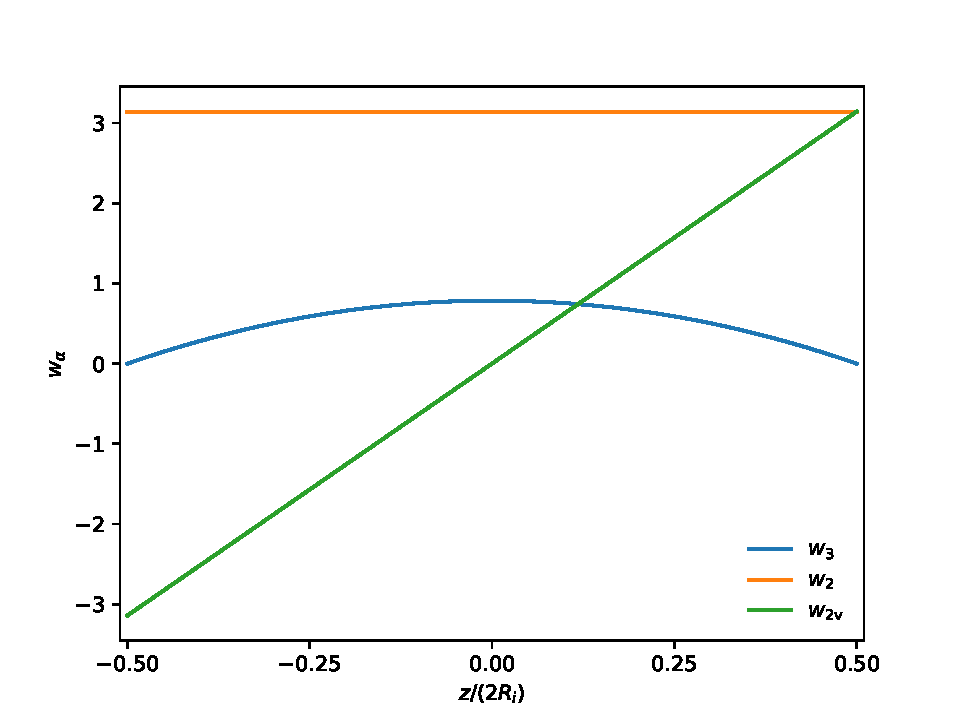
\includegraphics[width=0.49\textwidth]{gfx/planar_weights}
  \caption{Planar weight functions.}
  \label{fig:planar_weights}
\end{figure}

\subsubsection{Weight functions for spherical geometry}

For the shperical geometry $\rho \lb \mathbf{r} \rb = \rho \lb r \rb $,
and the weigth functions can be integrated for the angle dimensions.

\begin{equation}
  W_v \lb r \rb = \underset{-\infty}{\overset{\infty}{\int}} \underset{-\infty}{\overset{\infty}{\int}} dx dy w_v \lb \sqrt{x^2 + y^2 + z^2} \rb = 4 \pi \underset{\abs{r}}{\overset{\infty}{\int}} dr r^2  w_v \lb r \rb
\end{equation}

\todo{TODO}


\subsection{The White Bear functional}
\label{sec:fmt2}
The reduced Helmholtz energy of the White Bear functional with derivatives is:

\begin{align}
  \Phi^\WB =& -n_0 \ln \lb 1 - n_3 \rb +
              \frac{n_1 n_2 - \vc{n}_1 \cdot \vc{n}_2}{1 - n_3}\nonumber \\
  &+ \lb n_2^3 - 3 n_2 \vc{n}_2 \cdot \vc{n}_2 \rb \frac{ n_3 + \lb 1 - n_3 \rb ^2 \ln \lb 1 - n_3 \rb}{36\pi n_3^2 \lb 1 - n_3 \rb^2}
\end{align}

\begin{align}
  \pd{\Phi^\WB}{n_0} &= -\ln \lb 1 - n_3 \rb \\
  \pd{\Phi^\WB}{n_1} &= \frac{n_2}{1 - n_3} \\
  \pd{\Phi^\WB}{n_2} &= \frac{n_1}{1 - n_3} + \lb n_2^2 - \vc{n}_2 \cdot \vc{n}_2 \rb \frac{ n_3 + \lb 1 - n_3 \rb ^2 \ln \lb 1 - n_3 \rb}{12\pi n_3^2 \lb 1 - n_3 \rb^2} \\
  \pd{\Phi^\WB}{n_3} &= \frac{n_0}{1 - n_3} +
  \frac{n_1 n_2 - \vc{n}_1 \cdot \vc{n}_2}{\lb 1 - n_3 \rb^2} \nonumber \\
  & + \lb n_2^3 - 3 n_2 \vc{n}_2 \cdot \vc{n}_2 \rb \biggl( \frac{n_3 \lb 5 - n_3 \rb - 2}{36\pi n_3^2 \lb 1 - n_3 \rb^3} - \frac{\ln \lb 1 - n_3 \rb}{18\pi n_3^3} \biggr) \\
  \pd{\Phi^\WB}{\vc{n}_1} &=  - \frac{\vc{n}_2}{1 - n_3} \\
  \pd{\Phi^\WB}{\vc{n}_2} &=  -\frac{\vc{n}_1}{1 - n_3} - n_2 \vc{n}_2 \frac{ n_3 + \lb 1 - n_3 \rb ^2 \ln \lb 1 - n_3 \rb}{6\pi n_3^2 \lb 1 - n_3 \rb^2}
\end{align}

\subsection{The White Bear Mark II functional}
\label{sec:fmt2}
The reduced Helmholtz energy of the White Bear Mark II functional with derivatives is:

\begin{align}
  \Phi^\WBII =& -n_0 \ln \lb 1 - n_3 \rb +
  \lb n_1 n_2 - \vc{n}_1 \cdot \vc{n}_2 \rb \frac{1 + \frac{1}{3} \phi_2\lb n_3 \rb}{1 - n_3} \nonumber \\
  &+ \lb n_2^3 - 3 n_2 \vc{n}_2 \cdot \vc{n}_2 \rb\frac{ 1 - \frac{1}{3} \phi_3\lb n_3 \rb }{24\pi \lb 1 - n_3 \rb^2}
\end{align}
with,
\begin{align}
  \phi_2\lb n_3 \rb =& \frac{1}{n_3}\lb 2 n_3 - n_3^2 + 2\lb 1-n_3 \rb\ln \lb 1 - n_3 \rb \rb \\
  \phi_3\lb n_3 \rb =& \frac{1}{n_3^2}\lb 2 n_3 - 3n_3^2 + 2n_3^3 + 2\lb 1-n_3 \rb^2\ln \lb 1 - n_3 \rb \rb
\end{align}

\begin{align}
  \od{\phi_2}{n_3} =&  - 1 - \frac{2}{n_3} - \frac{2\ln \lb 1 - n_3 \rb}{n_3^2} \\
  \od{\phi_3}{n_3} =& -\frac{4 (1 - n_3) \ln \lb 1 - n_3\rb}{n_3^3}  - \frac{4}{n_3^2} + \frac{2}{n_3} + 2
\end{align}


\begin{align}
  \pd{\Phi^\WBII}{n_0} &= -\ln \lb 1 - n_3 \rb \\
  \pd{\Phi^\WBII}{n_1} &= \frac{n_2 \lb 1 + \frac{1}{3} \phi_2 \rb}{1 - n_3} \\
  \pd{\Phi^\WBII}{n_2} &= \frac{n_1 \lb 1 + \frac{1}{3} \phi_2 \rb}{1 - n_3} + \frac{\lb n_2^2 - \vc{n}_2 \cdot \vc{n}_2 \rb \lb 1 - \frac{1}{3} \phi_3 \rb}{8\pi \lb 1 - n_3 \rb^2} \\
  \pd{\Phi^\WBII}{n_3} &= \frac{n_0}{1 - n_3} +
                         \lb n_1 n_2 - \vc{n}_1 \cdot \vc{n}_2 \rb \biggl( \frac{\frac{1}{3} \od{\phi_2}{n_3}}{1 - n_3}  + \frac{1 + \frac{1}{3} \phi_2}{\lb 1 - n_3 \rb^2} \biggr) \nonumber \\
                         &+\frac{\lb n_2^3 - 3 n_2 \vc{n}_2 \cdot \vc{n}_2\rb}{24\pi \lb 1 - n_3 \rb^2} \biggl( - \frac{1}{3} \od{\phi_3}{n_3}  + \frac{ 2  \lb 1 - \frac{1}{3} \phi_3 \rb }{1 - n_3}\biggr) \\
  \pd{\Phi^\WBII}{\vc{n}_1} &=  - \frac{\vc{n}_2 \lb 1 + \frac{1}{3} \phi_2 \rb}{1 - n_3} \\
  \pd{\Phi^\WBII}{\vc{n}_2} &=  - \frac{\vc{n}_1 \lb 1 + \frac{1}{3} \phi_2 \rb}{1 - n_3} - \frac{n_2 \vc{n}_2\lb 1 - \frac{1}{3} \phi_3 \rb}{4\pi \lb 1 - n_3 \rb^2}
\end{align}

\subsection{The chain rule, convolutions and Fourier transforms}
The last term in the functional derivative (Eq.~\ref{eq:sol}) must for the hard-sphere term be expanded by use of the chain rule:
\begin{equation}
  \beta\frac{\delta F^{\text{hs}}\left[\left\{\rho_i\right\}\right]}{\delta\rho_j\left(\mathbf{r}\right)}
  =\sum_\alpha\frac{\partial\Phi^{\text{hs}}}{\partial n_\alpha\lb\mathbf{r}^\prime\rb}\frac{\delta n_\alpha\left(\mathbf{r}^\prime\right)}{\delta \rho_j\lb\mathbf{r}\rb}
\end{equation}
Furthermore, it can be shown that~\cite{stierle2020a}:
\begin{equation}
\frac{\delta n_\alpha\left(\mathbf{r}^\prime\right)}{\delta \rho_j\lb\mathbf{r}\rb}=w_j^\alpha\lb\mathbf{r}-\mathbf{r}^\prime\rb
\end{equation}
which gives:
\begin{equation}
  \beta\frac{\delta F^{\text{hs}}\left[\left\{\rho_i\right\}\right]}{\delta\rho_j\left(\mathbf{r}\right)}=\sum_\alpha\frac{\partial \Phi^{hs}}{\partial n_\alpha} \circledast w_j^\alpha
  \label{eq:conv2}
\end{equation}
which is a convolution of the derivative of the reduced Helmholtz density. Furthermore, the first term in the product is a function of the weighted densities, which are also convolutions (see Eq.~\ref{eq:wrho}). While convolutions can, in principle, be calculated by performing the intergrals in question numerically, it is both faster and more accurate to use fourier space transforms to do this task. The idea here is that while the convolution is an integral in real space, it is a product between two fourier transformed functions in Fourier space. The weighted density, for instance, can be calculated by:

\begin{equation}
  \begin{split}
    n_\alpha\left(\mathbf{r}\right)&=\sum_i^{N_c}\rho_i \lb\mathbf{r}\rb \circledast w_i^\alpha\lb\mathbf{r}\rb \\
    &= \mathscr{F}^{-1}\left[\mathscr{F}\left[\rho_i\lb\mathbf{r}\rb\right]\mathscr{F}\left[w_i^\alpha\lb\mathbf{r}\rb\right]\right]\\
    &= \mathscr{F}^{-1}\left[\hat{\rho}_i\left(\mathbf{k}\right)\hat{w}_i^\alpha\left(\mathbf{k}\right)\right]\\
  \end{split}
  \label{eq:Fourier}
\end{equation}

where $\hat{}$ refers to the transform of the respective quantity.

\subsubsection{Analytic representation of the transformed weight functions}
The convolutions above are all taken with respect to the weight functions, $w_i^\alpha$. The transforms of these functions can be computed analytically. The analytical expressions depend on which transform that is used. For the Fourier transform, they are:
\begin{eqnarray}
 &&\hat{w}_i^0\lb\mathbf{k}\rb=j_0\left(2\pi R_i|\mathbf{k}|\right) \label{eq:af1}\\
 &&\hat{w}_i^1\lb\mathbf{k}\rb= R_ij_0\left(2\pi R_i|\mathbf{k}|\right)\\
 &&\hat{w}_i^2\lb\mathbf{k}\rb= 4\pi R_i^2j_0\left(2\pi R_i|\mathbf{k}|\right)\\
 &&\hat{w}_i^3\lb\mathbf{k}\rb= \frac{4}{3}\pi R_i^3\left(j_0\left(2\pi R_i|\mathbf{k}|\right)+j_2\left(2\pi R_i|\mathbf{k}|\right) \right)\\
 &&\hat{w}_i^{V1}\lb\mathbf{k}\rb= \frac{-i\mathbf{k}}{2R_i}\hat{w}_i^3\lb\mathbf{k}\rb\\
 &&\hat{w}_i^{V2}\lb\mathbf{k}\rb=-i2\pi\mathbf{k}\hat{w}_i^3\lb\mathbf{k}\rb \label{eq:afN}
\end{eqnarray}
Here, $j_z$ is the Bessel functions of first kind of order $z$, $\mathbf{k}$ is the coordinate in Fourier space and $R_i$ is the hard-sphere diameter of component $i$ which is just a constant.
%For the Sine transform, the analytical expressions are:
%\begin{eqnarray}
% &&\hat{w}_i^0\lb\mathbf{k}\rb=\frac{\sin{\left(2\pi R_i\left|\mathbf{k}\right|\right)}}{2\pi R_i\left|\mathbf{k}\right|} \\
% &&\hat{w}_i^1\lb\mathbf{k}\rb=\frac{\sin{\left(2\pi R_i\left|\mathbf{k}\right|\right)}}{2\pi\left|\mathbf{k}\right|}\\
% &&\hat{w}_i^2\lb\mathbf{k}\rb= \dfrac{2R_i\sin{\left(2\pi R_i\left|\mathbf{k}\right|\right)}}{\left|\mathbf{k}\right|}\\
% &&\hat{w}_i^3\lb\mathbf{k}\rb= \frac{1}{2\pi^2\left|\mathbf{k}\right|^3}\left(\sin{\left(2\pi R_i\left|\mathbf{k}\right|\right)}-2\pi R_i\left|\mathbf{k}\right|\sin{\left(2\pi R_i\left|\mathbf{k}\right|\right)}\right)\\
% &&\hat{w}_i^{V1}\lb\mathbf{k}\rb=\frac{-i\mathbf{k}}{2R_i}\hat{w}_i^3\lb\mathbf{k}\rb \\
% &&\hat{w}_i^{V2}\lb\mathbf{k}\rb=-i2\pi\mathbf{k} \hat{w}_i^3\lb\mathbf{k}\rb
%\end{eqnarray}

\subsubsection{Minimum number of convolutions for efficient computations}
From a numerical point of view, we would like to perform as few convolutions in Fourier space as possible. Looking at Eq.~\ref{eq:af1}-\ref{eq:afN}, we see that:
\begin{eqnarray}
  &&\hat{w}_i^0=\frac{\hat{w}_i^2}{4\pi R_i^2} \\
  &&\hat{w}_i^1=\frac{\hat{w}_i^2}{4\pi R_i} \\
  &&\hat{w}_i^{V1}=\frac{\hat{w}_i^{V2}}{4\pi R_i} 
\end{eqnarray}
where $R_i$ is a constant. This means that we only need to perform three convolutions for each component to compute the weighted densities, for $n_{2,i}$, $n_{3,i}$ and $n_{V2,i}$ (see Eq.~\ref{eq:wrho}). then the rest follow from:
\begin{eqnarray}
  &&n_{0,i}=\frac{n_{2,i}}{4\pi R_i^2} \\
  &&n_{1,i}=\frac{n_{2,i}}{4\pi R_i} \\
  &&n_{V1,i}=\frac{n_{V2,i}}{4\pi R_i} 
\end{eqnarray}
Furthermore, we also need to compute convolutions in Eq.~\ref{eq:conv2}, and we can use the same procedure here, where:
\begin{equation}
  \sum_\alpha\frac{\partial \Phi^{hs}}{\partial n_\alpha} \circledast w_j^\alpha= \Phi_{2,j,\text{eff}}^{hs} \circledast w_j^2+
\frac{\partial \Phi^{hs}}{\partial n_{3}} \circledast w_j^3+
  \Phi_{V2,j,\text{eff}}^{hs} \circledast w_j^{V2}
\end{equation}
where
\begin{eqnarray}
&&\Phi_{2,i,\text{eff}}^{hs}=\frac{1}{4\pi R_i^2}\frac{\partial \Phi^{hs}}{\partial n_0}+\frac{1}{4\pi R_i}\frac{\partial \Phi^{hs}}{\partial n_1}+\frac{\partial \Phi^{hs}}{\partial n_2} \\
&&\Phi_{2V,i,\text{eff}}^{hs}=\frac{1}{4\pi R_i}\frac{\partial \Phi^{hs}}{\partial n_{V1}}+\frac{\partial \Phi^{hs}}{\partial n_{V2}}
\end{eqnarray}

\subsection{Fourier transforms}
The challenging aspect of solving the DFT is to compute the convolution integrals. This is done most efficiently and probably accurately in fourier space, where convolution integrals reduce to products between Fourier transforms, as shown in Eq.~\ref{eq:Fourier}. The problem of using the Fourier transform is that it assumes that your profile is a periodic signal, and will hence use information at the end of the domain when computing the convolution at the other end of the domain. To circumvent this, one must employ padding at the start and at the end of the domain, which essentially extrapolates the profiles. It is not always straightforward what this extrapolation should be. To avoid this padding, one uses instead Cosine and Sine transforms. In fact, the Fourier transform is a sum:

\begin{equation}
\mathscr{F}(f(\mathbf{r}))=\mathscr{C}(f(\mathbf{r}))-i\mathscr{S}(f(\mathbf{r}))
\end{equation}
where $\mathscr{C}$ and $\mathscr{S}$ are the cosine and sine transforms respectively. We shall next exploit that for even functions ($f(\mathbf{r})=f(-\mathbf{r})$), only the cosine transform is non-zero, and for odd functions ($f(\mathbf{r})=f(-\mathbf{r})$), only the sine transform is zero. The inverse transforms follow the same symmetry. We shall use the sine and cosine transforms for three geometries, planar, cylindrical and spherical. The good thing about the sine and cosine transforms is that they only go from 0 to infinity, meaning that they assume a certain symmetry for the rest of the domain at e.g. the centre (0), which means that we don't need padding, which is very convenient.

Moreover, if a different transform is used for the inverse transform than the transform, the grid has to be ``rolled'' due to a use of a different indexing for the cosine and sine transforms, as explained nicely in Sec.~4 of the paper by Stierle et al.~\cite{stierle2020a}, which we refer to for further details on this. For derivation of how the full fast Fourier transform can be replaced by sine and cosine transforms, we refer to Appendix B of the supplementary information of Ref.~\cite{stierle2020a}. Due to its nice symmetry fitting for many of the problems that we investigate, we employ the Type II sine and cosine transform (see~\cite{sinecosine_webpage} for details).

\subsubsection{Planar geometry}
As shown in Fig.~\ref{fig:planar_weights}, the scalar weight functions are even, and the vector valued weight functions are odd. That means that when we are computing the scalar weighted densities, we should use the cosine transform, and the sine transform for the vector weighted densities. Let us assume that there is only one relevant dimension, $r$, which is $k$ in Fourier space, and that $f(r)$ is a scalar function, and $\mathbf{f}(r)$ is a vector function, $w$ is the scalar weights, and $\mathbf{w}$ is  For a planar geometry we have that:

\begin{equation}
  f(r)\circledast w(r) = \mathscr{C}^{-1}\left(\mathscr{C}\left(f(r)\right)\hat{w}(k)\right)
  \label{eq:p1}
\end{equation}

\begin{equation}
  f(r)\circledast \mathbf{w}(r) = \mathscr{S}^{-1}\left(\mathscr{C}\left(f(r)\right)\hat{\mathbf{w}}(k)\right)\mathbf{e}_r
   \label{eq:p2}
\end{equation}

\begin{equation}
  \mathbf{f}(r)\circledast \mathbf{w}(r) = \mathscr{C}^{-1}\left(\mathscr{S}\left(\mathbf{f}(r)\right)\hat{\mathbf{w}}(k)\right)
   \label{eq:p3}
\end{equation}

where $\hat{}$ is the analytic Fourier transform, but it is important that the right grid is used depending on the inverse transform to be taken. Furthermore, $\mathbf{e}_r$ is the unit vector in the $r$ direction.

In the above relations, we have used that the scalar function, typically $\rho(r)$ or the functional derivatives with respect to the scalar weight are even functions ass well, which is due to the symmetry of the system around $r=0$. The vector functions that we consider in our case are $d\phi/d\mathbf{n}$, which have an odd symmetry (the sine transform should be used).

In Eq.~\ref{eq:p1}, we have a product between an even and an even function, which is even and the cosine transform should be used the whole way (the Fourier transform conserves the odd/even property).

In Eq.~\ref{eq:p2}, we have a product between an even function $f(r)$ and an odd function (the vector weight), which is odd. Since the product between the transformed quantities is odd, the inverse sine transform should be used.

In Eq.~\ref{eq:p3}, we have a product between an odd and an odd function, which is even. Hence, for both vector functions, the sine transforms should be used for the forward transform, and the cosine transform should be used for the backwards transform.

\subsubsection{Cylindrical geometry}
For a cylindrical grid, it is, per now, necessary to have a logarithmic grid and use the Hankel transform. We have also tried the Abel transform and combine that with a regular grid, but that did not give a satisfactory accuracy as the forward and backward transform did not properly recover a sharp density profile that was used as an example. Essentially more work is needed there.

To be filled in.

\subsubsection{Spherical geometry}
In the Fourier transform in spherical coordinates, the integration over angles can be done analytically, and the transform of an (even) scalar function is:
\begin{equation}
  f(r)\circledast w(r) = \frac{1}{r}\mathscr{S}^{-1}\left(\mathscr{S}\left(f(r)r\right)\hat{w}(k_r)\right)
  \label{eq:s1}
\end{equation}

\begin{equation}
  f(r)\circledast \mathbf{w}(r) = \mathbf{e}_r\left(\frac{1}{r^2}\mathscr{S}^{-1}\left(\mathscr{S}\left(f(r)r\right)\hat{w}^*(k_r)\right)-\frac{1}{r}\mathscr{C}^{-1}\left(\mathscr{S}\left(f(r)r\right)2\pi w_r\hat{w}^*(k_r)\right)\right)
   \label{eq:s2}
\end{equation}

\begin{equation}
  \mathbf{f}(r)\circledast \mathbf{w}(r) = \frac{1}{r}\mathscr{S}^{-1}\left(\mathscr{C}\left(f_r(r)r\right)2\pi k_r\hat{w}^*(k_r)-\mathscr{S}\left(f_r\right)\hat{w}^*(k_r)\right)
   \label{eq:s3}
\end{equation}
where:
\begin{equation}
\mathbf{f}(r)=f_r\mathbf{e}_r
\end{equation}
and
\begin{equation}
\hat{\mathbf{w}}=-2\pi i k_r\hat{w}^*(k_r)\mathbf{e}_r
\end{equation}
and $k_r$ is the fourier space spatial variabel.

Since $f(r)$ is even in Eq.~\ref{eq:s1}, $rf(r)$ becomes odd, and the sine transform has to be used instead of the cosine transform (as in the planar case). Furthermore, since $w(r)$ is even, odd multiplied by even becomes odd, which means that the inverse sine transformation has to be used. The fourier transform of the weight function is the same for all coordinate systems (allthough the grid changes between cosine and sine transforms).

For Eqs.~\ref{eq:s2} and \ref{eq:s3}, we must keep in mind that while $\hat{\mathbf{w}}$ is odd, $\hat{w}^*$ is even. 


\section{Numerics}

Solving of the convolution integrals in the FMT and cDFT in real space
uses $\mathcal{O}\lb N^2 \rb$ operations, however according to the
convolution theorem the integrals can be done by Fourier
transformations, leading to only $\mathcal{O}\lb N \ln N \rb$
operations \cite{roth2010, knepley2010}. Different options for solving
the discrete fast Fourier transform (FFT) is available, FFTW (GNU
General Public License), FFTPACK (MIT) and Python FFT.

The common approach used when solving \cdft problems is Picard
iterations. Instead of using a successive substituting iteration,
$\tilde{\rho}^{(i)} \rightarrow \rho^{(i)}$, a mixing of the new
density with the original density is used to dampen the effect of the
new value, accordign to,
\begin{equation}
  \tilde{\rho}^{(i+1)}\lb z \rb = \alpha \rho^{(i)}\lb z \rb + \lb 1 - \alpha \rb \tilde{\rho}^{(i)}\lb z \rb.
\end{equation}
The main reason is to avoid $n_3$ values exceeding unity.

Often the Picard parameter is set to a fixed low value, typically
$\alpha=0.1$, resulting in slow convergence. However using a line
search requiring some decay in error is probably the best way to
implement the Picard iterations. \citet{roth2010} suggest using a
simple quadratic line search. \citet{roth2010} used the Grand
Potential $\Omega$, when evaluating the line
search. \cite{knepley2010} evaluated the
$\| \tilde{\rho}^{(i)} - \rho^{(i)} \|$ as a function of $\alpha$ and
found the minimum of a quadratic polynomial.

One simple way of accelerate the solution of the equilibrium density
profile is by extrapolation as used by \citet{ng1974}.

\cite{knepley2010} tested a Newton solver (using numerical
approximations for the differentials), but they report linear
convergence through most of the iteration steps. The use of
inefficient generation of differentials was also reported as an issue.

Looking at Equation \eqref{eq:dndrho} and \eqref{eq:c1_1d} we see that
differentiating Equation \eqref{eq:c1_1d} will require convolution of
the $\Phi_{\alpha\gamma}$ with
$w_\alpha \lb z^\prime - z_1\rb w_\gamma \lb z^\prime - z_2\rb$. The
latter will become a matrix constant matrix requiering a convolution
integral per element in the banded Jacobian. The matrix is constant
and only the inverse Fourier transform will require computuational
effort. Each of these elements will require CPU time similar to one
half Picard iteration. For example if there are 1000 grid cells over
the diameter of a particle, the generation of one Jacobian instance
will be similar to 500 Picard iterations.

Parallel solution for the Fourier transforms are simple using the FFTW library....

\subsubsection{Quadratures for the weight functions}
Integrating on a regular grid the integral can be made more accurate using a qudrature formula \todo{Cite},
\begin{align}
  \underset{z_N}{\overset{z_1}{\int}} dz^\prime f \lb z^\prime \rb g \lb z^\prime - z \rb =& \Delta z \biggl( \frac{3}{8} f_1 g_{i-1} + \frac{7}{6} f_2 g_{i-2} + \frac{23}{24} f_3 g_{i-3} + f_4 g_{i-4} \nonumber \\&+ \dots  + f_{N-3} g_{i-N+3} + \frac{23}{24} f_{N-2} g_{i-N+2} \nonumber \\&+ \frac{7}{6} f_{N-1} g_{i-N+1} + \frac{3}{8} f_{N-2} g_{i-N+2}.
\end{align}
The qudarature is implemeted by multipying the end weights with by the
quadrature weights.

The actual planar weight functions are visualized in Figure
\ref{fig:actual_planar_weights}.
\begin{figure}[tbp]
  \centering
  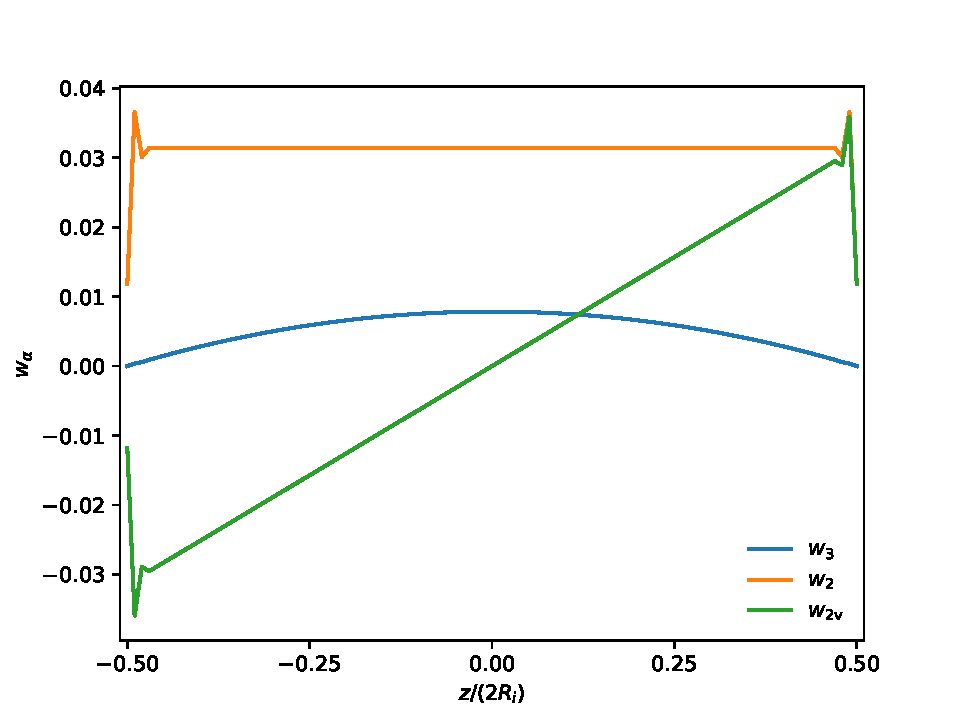
\includegraphics[width=0.49\textwidth]{gfx/actual_planar_weights}
  \caption{Actual planar weight functions.}
  \label{fig:actual_planar_weights}
\end{figure}

\section{Perturbation theory}
The canonical partition function,
\begin{equation}
  Q_N = \frac{1}{h^{3N}N!}\int d \mathbf{p}^N \int d \rvec^N e^{-\beta \mathcal{H}}
\end{equation}
Relation between Helmholtz energy and partition function,
\begin{equation}
  \label{eq:helm_statmec}
  F = -\kB T \ln Q_N
\end{equation}
Using a Hamiltonian,
\begin{equation}
  \mathcal{H} = \Phi \lb \rvec^N \rb + K\lb \pvec^N \rb + V_\external \lb \rvec^N \rb,
\end{equation}
where the kinetic energies is given from the moments,
\begin{equation}
  K\lb \pvec^N \rb = \overset{N}{\underset{i=1}{\sum}} \frac{\abs{\pvec_i}^2}{2 m}
\end{equation}
the partition function can be integrated with respect to the moments,
\begin{align}
  Q_N &= \frac{1}{h^{3N}N!}\int d \mathbf{p}^N e^{-beta + K\lb \pvec^N \rb } \int d \rvec^N e^{-\beta \lb \Phi \lb \rvec^N \rb + V_\external \lb \rvec^N \rb \rb} \nonumber \\
      &= \frac{1}{\Lambda^{3N}N!} \int d \rvec^N e^{-\beta \lb \Phi \lb \rvec^N \rb + V_\external \lb \rvec^N \rb \rb} \nonumber\\
  &= \frac{Z_N}{\Lambda^{3N}N!}
\end{align}
where $Z_N$ is the configurational integral, and $\Lambda$ is the
thermal de Broglie wavelength.

Having the perturbation potential
\begin{equation}
  \phi_\lambda \lb \rvec, \rvec^\prime \rb = \phi_0 \lb \rvec, \rvec^\prime \rb + \lambda \phi_\attractive \lb \rvec, \rvec^\prime \rb \quad 0 \le \lambda \le 1,
\end{equation}
where $\lambda$ is the perturbation strength, the potential energy felt between all particles is given by
\begin{equation}
\Phi \lb \rvec^N \rb = \overset{N}{\underset{j=1}{\sum}} \overset{N}{\underset{k>j}{\sum}} \phi_\lambda \lb \rvec, \rvec^\prime \rb
\end{equation}
The excess Helmholtz energy can be differentiated with respect to $\lambda$ using Equation \eqref{eq:helm_statmec},
\begin{equation}
  \label{eq:helm_expancion}
\beta \pd{F_\excess}{\lambda} = -\frac{1}{Z_N} \pd{Z_N}{\lambda} = \frac{\beta}{2} \int d \rvec \int d \rvec^\prime \rho_\lambda^{(2)}\lb \rvec, \rvec^\prime \rb \phi_\attractive \lb \rvec, \rvec^\prime \rb
\end{equation}
we can also describe the Helmholtz energy using ensemble average, $\langle \dots \rangle_\lambda$, for a system described by $\phi_\lambda$,
\begin{equation}
\beta \pd{F_\excess}{\lambda} = \langle \Phi^\prime \rangle_\lambda
\end{equation}
where $\pd{\Phi_\lambda}{\lambda} = \Phi_\lambda^\prime$. Integration yields,
\begin{equation}
\beta F_\excess = \beta F_0 + \overset{\lambda=1}{\underset{\lambda=0}{\int}} d \lambda \langle \Phi^\prime \rangle_\lambda
\end{equation}

In order to get ensemble averages over the reference system
$\lambda = 0$, the average can be expanded in $\lambda$ around
$\lambda = 0$.

Leading to
\begin{equation}
\beta F_\excess = \beta F_0 + \beta F_1 + \beta F_2 + \beta F_3 + \mathcal{O}\lb \beta^4 \rb
\end{equation}
where
\begin{align}
  \beta F_1 &= \beta \langle \Phi_\attractive  \rangle_0\\
  \beta F_2 &= -\frac{\beta^2}{2} \biggl[ \langle \Phi_\attractive^2  \rangle_0 - \langle \Phi_\attractive  \rangle_0^2 \biggr] \\
  \beta F_3 &= \frac{\beta^3}{3!} \bigg\langle \Phi_\attractive - \langle \Phi_\attractive  \rangle_0 \bigg\rangle^3
\end{align}

For pair-wise additive potentials we have,
\begin{equation}
  \label{eq:first_order_pert}
\frac{\beta F_1}{N} = \frac{\beta \rho}{2} \int  g_\lambda \lb r \rb \phi_\attractive \lb r \rb d r
\end{equation}
and to first order $g_\lambda = g_0$.

\section{Approaches used when extending \cdft to attractive fluids}

\subsection{Mean Field Theory (MFT)}
Under the MFT approximation, $g_ \approx 1$, and Equation
\eqref{eq:first_order_pert} simply becomes
\begin{equation}
  \label{eq:mft}
  \frac{\beta F_1}{N} = \frac{\beta \rho}{2} \phi_\attractive \lb r \rb d r
\end{equation}

For some reason it is common to use the WCA perturbation potential,
however the hard-sphere diameter seem to be independent of density.
\todo{Check if cDFT\_Package uses sigma=1 with WCA simulation....}

\subsection{Local density approximation (LDA)}
Under the LDA assumption the Helmholtz energy density of an
inhomogeneous system with density profile $\rho \lb r\rb$ is
calculated using the bulk phase Helmholtz energy density evaluated at
the value of the local density. This often work for surface tension
calculations, however adjacent to walls where the density oscillate
strongly and the local density can exceed the maximum packing fractions
this will be a problem.

\subsection{Weighted density approximation (WDA)}
The WDA uses locally weighted densities and evaluates the Helmholtz
energy functional with these densities. This methodology have proven
successful even for fluid to wall interacting systems.

\citet{sauer2017}
\citet{tarazona1984, tarazona1984a}

\subsection{Nonlocal perturbation theory (NLP)}
\citet{gloor2004}
\citet{gross2009}

\section{The PCP-SAFT \cdft}

\citet{sauer2017}

PC-SAFT \citet{gross2001}
Polar extensions
Quadruplole-Quadruplole:\citet{gross2005}
Dipole-dipole:\citet{gross2006}
Dipole-Quadruplole: \citet{vrabec2008}



\section{Analytial Fourier transforms of the weight functions}
\citet[Appendix B]{knepley2010} derives the analytical Fourier
transform for the weight functions.

\subsection{Planar geometry}
The weight functions in a planar geometry is derived in section
\ref{sec:planar_weights}. The weight functions can be transformed to
Fourier space according to the definition,
\begin{align}
  \label{eq:fourier}
  \hat{w}_\alpha^i \lb k \rb = \mathcal{F}\lb w_\alpha^i \lb z \rb \rb =& \overset{\infty}{\underset{-\infty}{\int}} dz w_\alpha^i \lb z \rb e^{-i k z} \nonumber \\
  =& \overset{\infty}{\underset{-\infty}{\int}} dz w_\alpha^i \lb z \rb \cos \lb k z \rb + i \overset{\infty}{\underset{-\infty}{\int}} dz w_\alpha^i \lb z \rb \sin \lb k z \rb
\end{align}

Since $w_3^i$ and $w_2^i$ are even functions, the Fourier transform
will be purely real valued, while $\mathbf{w}_2^i$ is odd and
therefore purly imaginary,
\begin{align}
  \hat{w}_3^i &=  \overset{\infty}{\underset{-\infty}{\int}} dz  \pi \lb R_i^2 - z^2 \rb \Theta \lb R_i - \abs{z} \rb \cos \lb k z \rb \nonumber \\
              &=  \pi \overset{R_i}{\underset{-R_i}{\int}} dz  \lb R_i^2 - z^2 \rb \cos \lb k z \rb  \nonumber \\
              &=  \frac{4 \pi}{k^3} \biggl( \sin \lb k R_i \rb - k R\cos \lb k R_i \rb \biggr) \label{eq:w_hat_3}
\end{align}

\begin{align}
  \hat{w}_2^i &=  \overset{\infty}{\underset{-\infty}{\int}} dz 2 \pi R_i \Theta \lb R_i - \abs{z} \rb \cos \lb k z \rb \nonumber \\
              &=  2 \pi R_i \overset{R_i}{\underset{-R_i}{\int}} dz  \cos \lb k z \rb  \nonumber \\
              &=  \frac{4 \pi R_i}{k} \sin \lb k R_i \rb \label{eq:w_hat_2}
\end{align}

\begin{align}
  \hat{\mathbf{w}}_2^i &=  i \overset{\infty}{\underset{-\infty}{\int}} dz 2 \pi \mathbf{z}  \Theta \lb R_i - \abs{z} \rb \cos \lb \mathbf{k} \cdot \mathbf{z} \rb \nonumber \\
                       &=  2 \pi i  \overset{R_i}{\underset{-R_i}{\int}} dz \mathbf{z}  \cos \lb \mathbf{k} \cdot \mathbf{z} \rb =  - 2 \pi i \mathbf{e}_k  \overset{R_i}{\underset{-R_i}{\int}} dz z  \cos \lb k z \rb \nonumber \\
                       &=  -\frac{4 \pi i}{k^2} \biggl( \sin \lb k R_i \rb - k R_i \cos \lb k R_i \rb \biggr) \mathbf{e}_k \label{eq:w_hat_2v}
\end{align}
Comparing equations \eqref{eq:w_hat_3}, \eqref{eq:w_hat_2} and \eqref{eq:w_hat_2v}, we see that the equation s \todo{.......}


\section{Bulk properties for hard spheres}

The excess pressure of the system is described as
\begin{equation}
  \label{eq:pressure}
  \beta p_{\excess} = -\pd{\beta \mathcal{F_{\excess}}}{V} = -\pd{\lb V \Phi \rb}{V} = -\Phi - V\underset{i=1}{\sum} \pd{\Phi}{n_{\alpha}}\pd{n_{\alpha}}{V} = -\Phi + \underset{i=1}{\sum} \pd{\Phi}{n_{\alpha}}n_{\alpha}
\end{equation}

The ideal pressure of the system is simply
\begin{equation}
  \beta p_{\ideal} = n_{0}.
\end{equation}

The excess chemical potential of the system is described as
\begin{equation}
  \label{eq:chem_pot}
  \hat{\mu}^i_{\excess} = \beta \mu^i_{\excess} = \pd{\beta \mathcal{F_{\excess}}}{N_i} = \pd{\lb V \Phi \rb}{N_i} = \pd{\Phi}{\rho_{i}} = \underset{\alpha}{\sum} \pd{\Phi}{n_{\alpha}}\pd{n_{\alpha}}{\rho_{i}}
\end{equation}

% \begin{equation}
%   \frac{\mu^\RF_{i,\bulk}}{\kB T} = \int \biggl(\frac{Z-1}{\rho_i} \biggr) d\rho_i + Z - 1
% \end{equation}

% \begin{align}
%   \pd{\Phi^\RF_\bulk}{\rho_i} =& - \ln \lb 1 - n_3 \rb + \frac{n_0}{ \lb 1 - n_3 \rb}\pd{n_3}{\rho_i} \nonumber \\ &+
%   \frac{n_2}{\lb 1 - n_3 \rb}\pd{n_1}{\rho_i} + \frac{n_1}{\lb 1 - n_3 \rb}\pd{n_2}{\rho_i} + \frac{n_1 n_2}{\lb 1 - n_3 \rb^2}\pd{n_3}{\rho_i} \nonumber \\ &+
%   \frac{3 n_2^2 }{24\pi \lb 1 - n_3 \rb^2}\pd{n_2}{\rho_i} + \frac{2 n_2^3 }{24\pi \lb 1 - n_3 \rb^3}\pd{n_3}{\rho_i}
% \end{align}
For the bulk limit we have
\begin{align}
  n_{0,\bulk} &= \overset{\NC}{\underset{i=1}{\sum}} \rho_{i,\bulk}\\
  n_{1,\bulk} &= \overset{\NC}{\underset{i=1}{\sum}} R_i \rho_{i,\bulk}\\
  n_{2,\bulk} &= 4 \pi \overset{\NC}{\underset{i=1}{\sum}} R_i^2 \rho_{i,\bulk}\\
  n_{3,\bulk} &= \frac{4 \pi}{3} \overset{\NC}{\underset{i=1}{\sum}} R_i^3 \rho_{i,\bulk}
\end{align}
and
\begin{align}
  \pd{n_{0,\bulk}}{\rho_{i,\bulk}} &= 1\\
  \pd{n_{1,\bulk}}{\rho_{i,\bulk}} &=  R_i\\
  \pd{n_{2,\bulk}}{\rho_{i,\bulk}} &= 4 \pi R_i^2\\
  \pd{n_{3,\bulk}}{\rho_{i,\bulk}} &= \frac{4 \pi}{3} R_i^3
\end{align}
leading to
\begin{equation}
  \beta \mu^i_{\excess,\bulk} = \pd{\Phi}{n_{0,\bulk}} + R_i \pd{\Phi}{n_{1,\bulk}} + 4 \pi R_i^2 \pd{\Phi}{n_{2,\bulk}} + \frac{4 \pi R_i^3}{3} \pd{\Phi}{n_{3,\bulk}}
\end{equation}

\subsection{The Rosenfeld functional}
In the bulk phase (delete vector weight contributions) the Rosenfeld functional reduces to
\begin{equation}
  \Phi^\RF_\bulk = -n_0 \ln \lb 1 - n_3 \rb +
  \frac{n_1 n_2}{1 - n_3} +
  \frac{n_2^3 }{24\pi \lb 1 - n_3 \rb^2}
\end{equation}
which is the scaled particle theory (SPT) Helmholtz energy equation
for mixtures. The SPT EOS is identical to the Percus–Yevick EOS.

The bulk differentials become,
\begin{align}
  \pd{\Phi^\RF}{n_{0,\bulk}} &= -\ln \lb 1 - n_{3,\bulk} \rb \\
  \pd{\Phi^\RF}{n_{1,\bulk}} &= \frac{n_{2,\bulk}}{1 - n_{3,\bulk}} \\
  \pd{\Phi^\RF}{n_{2,\bulk}} &= \frac{n_{1,\bulk}}{1 - n_{3,\bulk}} + \frac{n_{2,\bulk}^2}{8\pi \lb 1 - n_{3,\bulk} \rb^2} \\
  \pd{\Phi^\RF}{n_{3,\bulk}} &= \frac{n_{0,\bulk}}{1 - n_{3,\bulk}} +
  \frac{n_{1,\bulk} n_{2,\bulk}}{\lb 1 - n_{3,\bulk} \rb^2} +
  \frac{n_{2,\bulk}^3}{12\pi \lb 1 - n_{3,\bulk} \rb^3}
\end{align}

\begin{align}
  \beta p_{\excess} + \Phi =& \underset{i=1}{\sum} \pd{\Phi}{n_{\alpha}}n_{\alpha} \nonumber \\
  = & -n_{0,\bulk} \ln \lb 1 - n_{3,\bulk} \rb \nonumber \\
      &+ n_{1,\bulk}\frac{n_{2,\bulk}}{1 - n_{3,\bulk}} \nonumber \\
      &+ n_{2,\bulk} \biggl(\frac{n_{1,\bulk}}{1 - n_{3,\bulk}} + \frac{n_{2,\bulk}^2}{8\pi \lb 1 - n_{3,\bulk} \rb^2} \biggr) \nonumber \\
      &+ n_{3,\bulk} \biggl(\frac{n_{0,\bulk}}{1 - n_{3,\bulk}} + 
      \frac{n_{1,\bulk} n_{2,\bulk}}{\lb 1 - n_{3,\bulk} \rb^2} +
        \frac{n_{2,\bulk}^3}{12\pi \lb 1 - n_{3,\bulk} \rb^3} \biggr) \nonumber\\
    = & -n_{0,\bulk} \ln \lb 1 - n_{3,\bulk} \rb 
      + \frac{2n_{1,\bulk}n_{2,\bulk}}{1 - n_{3,\bulk}}
      + \frac{n_{2,\bulk}^3}{8\pi \lb 1 - n_{3,\bulk} \rb^2}  \nonumber \\
      &+ n_{3,\bulk} \biggl(\frac{n_{0,\bulk}}{1 - n_{3,\bulk}} + 
      \frac{n_{1,\bulk} n_{2,\bulk}}{\lb 1 - n_{3,\bulk} \rb^2} +
        \frac{n_{2,\bulk}^3}{12\pi \lb 1 - n_{3,\bulk} \rb^3} \biggr) \\
  \beta p_{\excess} &= \frac{n_{1,\bulk}n_{2,\bulk}}{1 - n_{3,\bulk}}
      + \frac{n_{2,\bulk}^3}{8\pi \lb 1 - n_{3,\bulk} \rb^2}  \nonumber \\
      &+ n_{3,\bulk} \biggl(\frac{n_{0,\bulk}}{1 - n_{3,\bulk}} + 
      \frac{n_{1,\bulk} n_{2,\bulk}}{\lb 1 - n_{3,\bulk} \rb^2} +
        \frac{n_{2,\bulk}^3}{12\pi \lb 1 - n_{3,\bulk} \rb^3} \biggr) \nonumber\\
                            &- \frac{n_{2,\bulk}^3 }{24\pi \lb 1 - n_{3,\bulk} \rb^2} \nonumber\\
                            &= \frac{n_{0,\bulk}n_{3,\bulk}}{\lb 1 - n_{3,\bulk} \rb} + \frac{n_{1,\bulk} n_{2,\bulk}}{\lb 1 - n_{3,\bulk} \rb^2} + \frac{n_{2,\bulk}^3}{12 \pi\lb 1 - n_{3,\bulk} \rb^3}
\end{align}
Adding the ideal contribution, $\beta p_{\ideal} = n_{0,\bulk}$, and
dividing by $n_{0,\bulk}$ we get the compressibillity of the SPT EOS,
\begin{equation}
  z^\RF_\bulk = \frac{p}{n_0 \kB T} = \frac{1}{\lb 1 - n_3 \rb} + \frac{n_1 n_2}{n_0} \frac{1}{\lb 1 - n_3 \rb^2} + \frac{n_2^3}{12 \pi n_0} \frac{1}{\lb 1 - n_3 \rb^3},
\end{equation}
and for a singel component the equation reduces to
\begin{equation}
  z^\RF_{\bulk,\pure} = \frac{1 + n_3 + n_3^2}{\lb 1 - n_3 \rb^3}.
\end{equation}

For the pure fluid, using $\eta = n_{3,\bulk}$ and \eqref{eq:chem_pot} we get,
\begin{align}
  \hat{\mu}^\pure_{\excess,\bulk} =& -\ln \lb 1 - \eta \rb + \frac{3 \eta}{1 - \eta} + \frac{3 \eta}{1 - \eta} + \frac{36\pi\eta^2}{8\pi \lb 1 - \eta \rb^2}\nonumber \\
  & +\frac{\eta}{1 - \eta} +
  \frac{3 \eta^2}{\lb 1 - \eta \rb^2} +
    \frac{36\pi\eta^3}{12\pi \lb 1 - \eta \rb^3}\nonumber \\
   =&-\ln \lb 1 - \eta \rb + \frac{7 \eta}{1 - \eta} + \frac{15\eta^2}{2\lb 1 - \eta \rb^2}+
      \frac{3\eta^3}{\lb 1 - \eta \rb^3}\nonumber \\
  =&\frac{14\eta - 13\eta^2 + 5\eta^3}{2\lb 1 - \eta \rb^3}-\ln \lb 1 - \eta \rb
\end{align}

\section{Thermopack properties}
The cDFT code use reduced units, and the spatial dimension is reduced
with respect to the hard-sphere diameter of the first component in the
mixture. The gemoetry is therefore defined by the widt $L$ in reduced
units, and the actual widht is therefore $L d_{11}$. The component densities are
\begin{equation}
  \rho_{i}^* = \frac{N_id_{11}^3}{V}.
\end{equation}
The temperature is also given from component 1 and
\begin{equation}
  T^* = \frac{\kB T}{\epsilon_{11}}.
\end{equation}

\subsection{Bulk fluid}
The thermopack interface use functions of temperature, volume and mol
numbers, ($T, V, \mathrm{n}$). When calculating thermopack properties,
the densities must be converted to Thermopack units
\begin{equation}
  \mathrm{\rho}_n = \mathrm{\rho}^*\frac{1}{\NA d_{11}^3}.
\end{equation}
Thermopack can then be evaluated using $V=1.0$ and $\mathrm{\rho}$, or
the densities cam be converted to mol numbers and specific volume.

\begin{align}
  \beta A \lb T, V, \mathrm{n} \rb &= \frac{1}{V}\beta A \lb T, 1, \mathrm{\rho} \rb \\
  \frac{1}{V}\beta A \lb T, 1, \mathrm{\rho} \rb\frac{1}{\sum \rho_i} &= \beta A \lb T, 1, \mathrm{\rho} \rb\frac{1}{\sum n_i}\nonumber \\
  &= a \lb T, \mathrm{\rho} \rb
\end{align}

The \excess reduced chemical potential is given from thermopack as
\begin{equation}
  \beta \mu_{i}^\excess = \beta\pd{A^\excess}{N_i} =
  \beta \pd{A^\excess \lb T, V, \mathrm{n} \rb}{n_i} \pd{n_i}{N_i} = \frac{1}{R T}\pd{A^\excess \lb T, V, \mathrm{n} \rb}{n_i}.
\end{equation}

The \excess compressibillity from thermopack is given as
\begin{equation}
  z^\excess = \frac{P^\excess}{\underset{i}{\sum} \rho_{n,i} R T}
\end{equation}

\subsection{Dispersion functional differentials}
Thermopack implements the dispersion contribution as
\begin{equation}
  a_\disp\lb T, V, \mathrm{n} \rb = \frac{A_\disp\lb T, V, \mathrm{n} \rb}{n R T}.
\end{equation}
The \cdft code need differentials for the functional $\beta \rho^* a_\disp\lb \rho^* \rb$,
\begin{align}
  \pd{\lb \rho a_\disp\lb \rho^* \rb \rb}{\rho_i} & = a_\disp +  \rho^* \pd{a_\disp}{\rho_i^*} \nonumber \\
                                                  & = a_\disp +  \rho^* \pd{a_\disp}{\rho_{n,i}} \pd{\rho_{n,i}}{\rho_i^*} \nonumber \\
                                                  & = a_\disp +  \rho^* \pd{a_\disp}{\rho_{n,i}} \frac{1}{\NA d_{11}^3}\nonumber \\
                                                  & = a_\disp +  \rho_n \pd{a_\disp}{\rho_{n,i}}.
\end{align}
Thermopack can then be evaluated setting $V=1.0$ and
$\mathrm{n}=\mathrm{\rho}_n$.
\clearpage
\bibliographystyle{plainnat}
\bibliography{./DFT.bib,./HardSphere.bib,./PC-SAFT.bib}

\end{document}

%%% Local Variables: 
%%% mode: latex
%%% TeX-master: t
%%% ispell-local-dictionary: "british"
%%% End: 
